\documentclass{article}
\usepackage[utf8]{inputenc}

\title{Um modelo para a COVID-19}
\author{Daniel Girardi e Marcelo Dallangol}
\date{March 2020}

\usepackage{natbib}
\usepackage{graphicx}

\begin{document}


\maketitle

\section{Modelo}

Vamos utilizar um modelo determinístico baseado em 10 compartimentos e com variáveis em valores absolutos. Ou seja, o tamanho da população e número de infectados terão valores absolutos. Essa opção visa a comparação direta entre os valores obtidos pelo modelo com os dados oriundos dos órgãos de saúde. 

% \subsection{Saudáveis (S)}
% A fração $\delta$ de \textit{Saudáveis} (aqueles que não estão seguindo a quarentena rigorosamente) podem ser contaminados pelos \textit{Infectados} (I) e \textit{Infectados Graves} ($I_g$). Neste caso, eles tornan-se \textit{Expostos}. 
% \begin{equation}
% 	\frac{dS}{dt}= -S\delta(\alpha_i I +\alpha_{ig}I_g)
% \end{equation}
% \begin{figure}[!h]
% 	\centering
% 	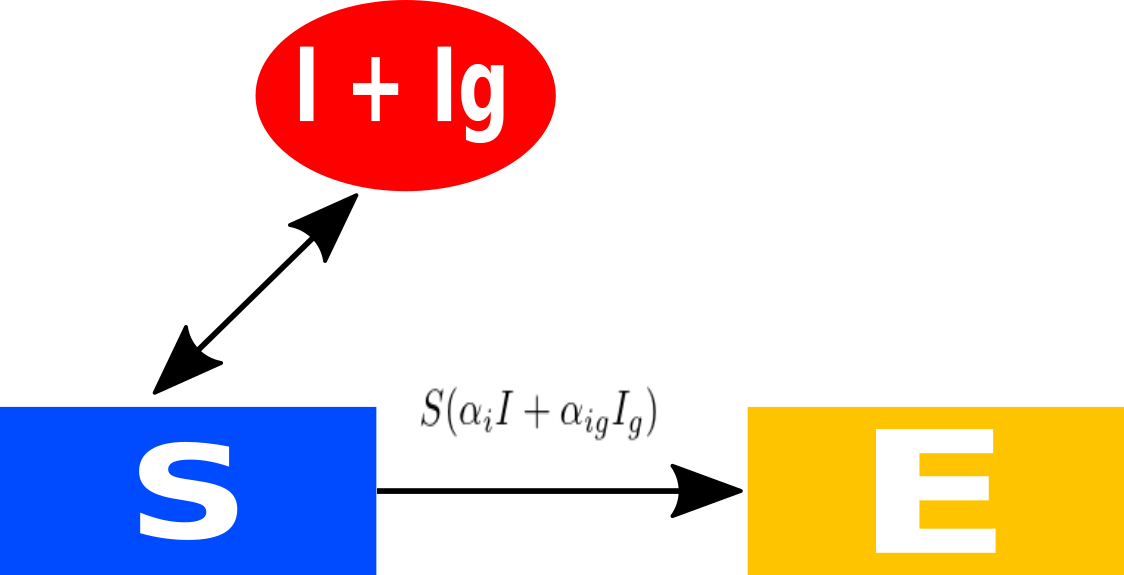
\includegraphics[scale=0.4]{covidS}
% 	\caption{Diagrama da equação dos Saudáveis.}
% 	\label{fig:universe}
% \end{figure}

% \subsection{Expostos (E)}
% Os \textit{Expostos} aumentam conforme há a contaminação dos \textit{Saudáveis} e com o tempo evoluem a uma taxa $\beta$ para o estado \textit{Infectado}.

% \begin{equation}
% 	\frac{dE}{dt}= S(\alpha_i I +\alpha_{ig}I_g) - \beta E
% \end{equation}
% \begin{figure}[!h]
% 	\centering
% 	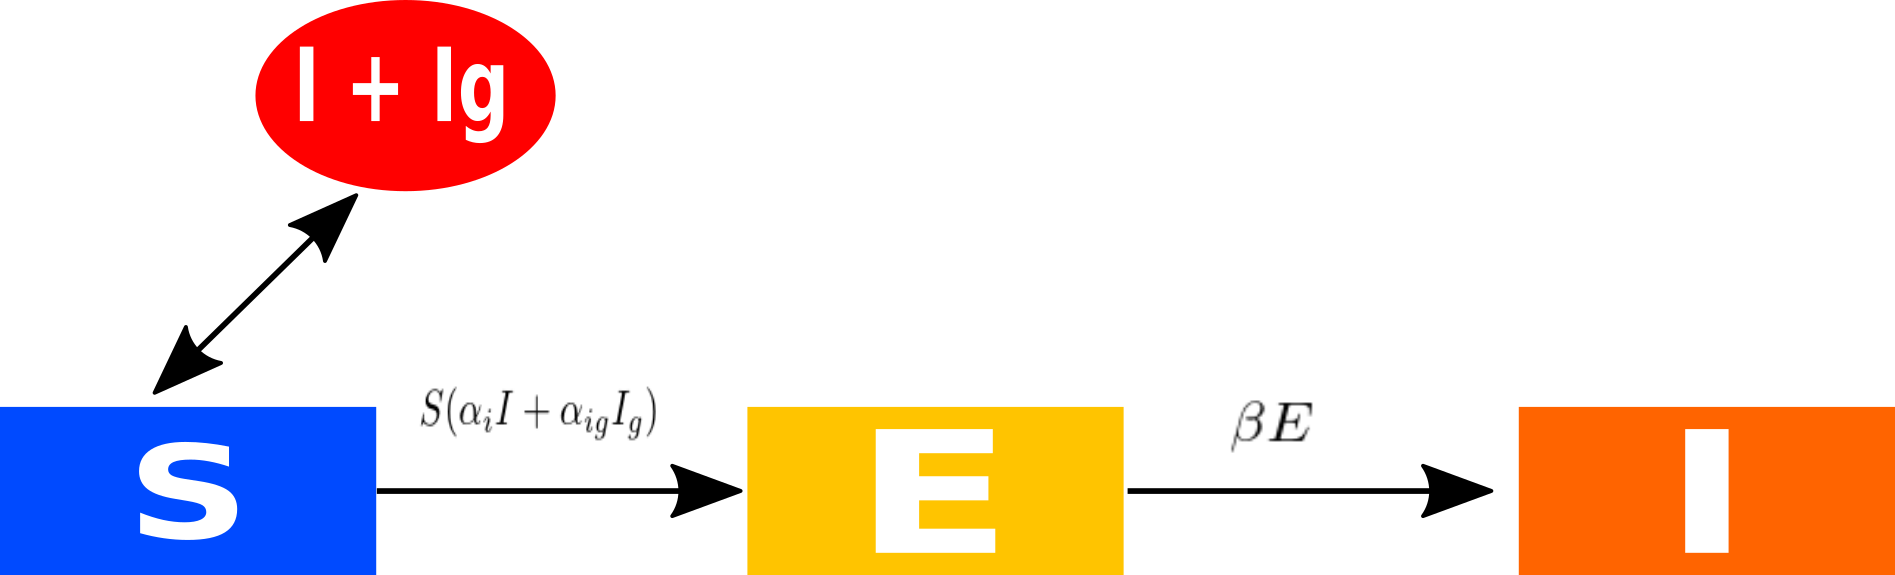
\includegraphics[scale=0.4]{covidE}
% 	\caption{Diagrama da equação dos Expostos.}
% 	\label{fig:universe}
% \end{figure}

% \subsection{Infectados (I)}
% Esses são os que eram \textit{Expostos}, mas evoluíram para o estado ativo da doença. \textbf{Por definição}, estes são os indivíduos que podem contaminar indivíduos saudáveis, não são apenas os que foram testados como positivo para COVID. Estes podem evoluir a uma taxa $\lambda_I$ para curados ou evoluir a uma taxa $\zeta$ para \textit{Infectados no estado Grave}.
% \begin{equation}
% 	\frac{dI}{dt}= \beta E -\lambda_i I - \zeta I
% \end{equation}
% \begin{figure}[!h]
% 	\centering
% 	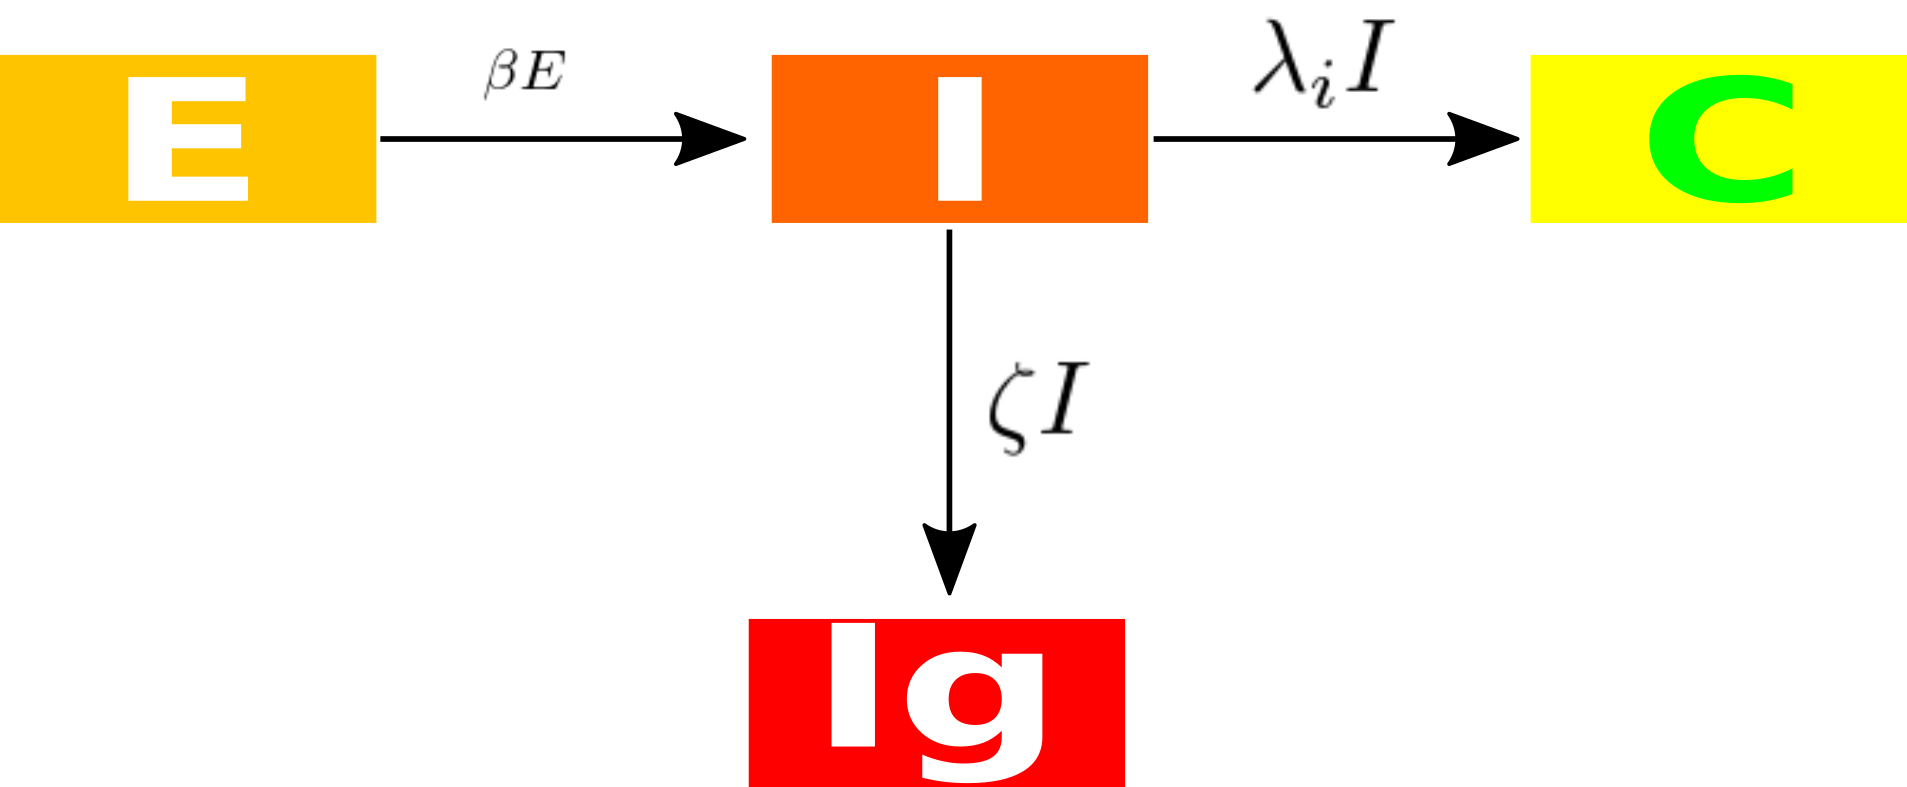
\includegraphics[scale=0.4]{covidI}
% 	\caption{Diagrama da equação dos Infectados.}
% 	\label{fig:universe}
% \end{figure}

% \subsection{Infectados Graves ($I_G$)}
% São os que manifestaram o quadro grave e que necessitam de internação hospitalar. Contudo, os hospitais possuem uma capacidade de postos de internação que são definidos pelo número de leitos comuns ($\kappa_L$) mais o número de leitos de UTI ($\kappa_U$). Portanto, uma parcela $\gamma$ destes, irão procurar os hospitais mas só serão recebidos de acordo com a disponibilidade de leitos $(1-\frac{H_l+H_u+H_{lg}+H_{lv}}{\kappa_l+\kappa_u})$. Se a soma te todos os hospitalizados  $H_l+H_u+H_{lv}+H_{lg}$ (leito comum, UTI, leito comum com ventilação mecânica e leito comum em estado grave) for igual a capacidade total dos hospitais $\kappa_l+\kappa_u$, então esse indivíduo continuará no estado $I_G$. Neste estado, os indivíduos morrem a uma taxa $\mu_{ig}$ e se curam a uma taxa $\lambda_{ig}$. Do ponto de vista médico, sabe-se que $\mu_{ig}$ é a maior taxa de morte e $\lambda_{ig}$ a menor taxa de cura.

% \begin{equation}
% 	\frac{dI_G}{dt}= \zeta I -(1-\frac{H_l+H_u+H_{lg}+H_{lv}}{\kappa_l+\kappa_u})\gamma I_G - \lambda_{ig} I_G - \mu_{ig} I_G
% \end{equation}
% \begin{figure}[!h]
% 	\centering
% 	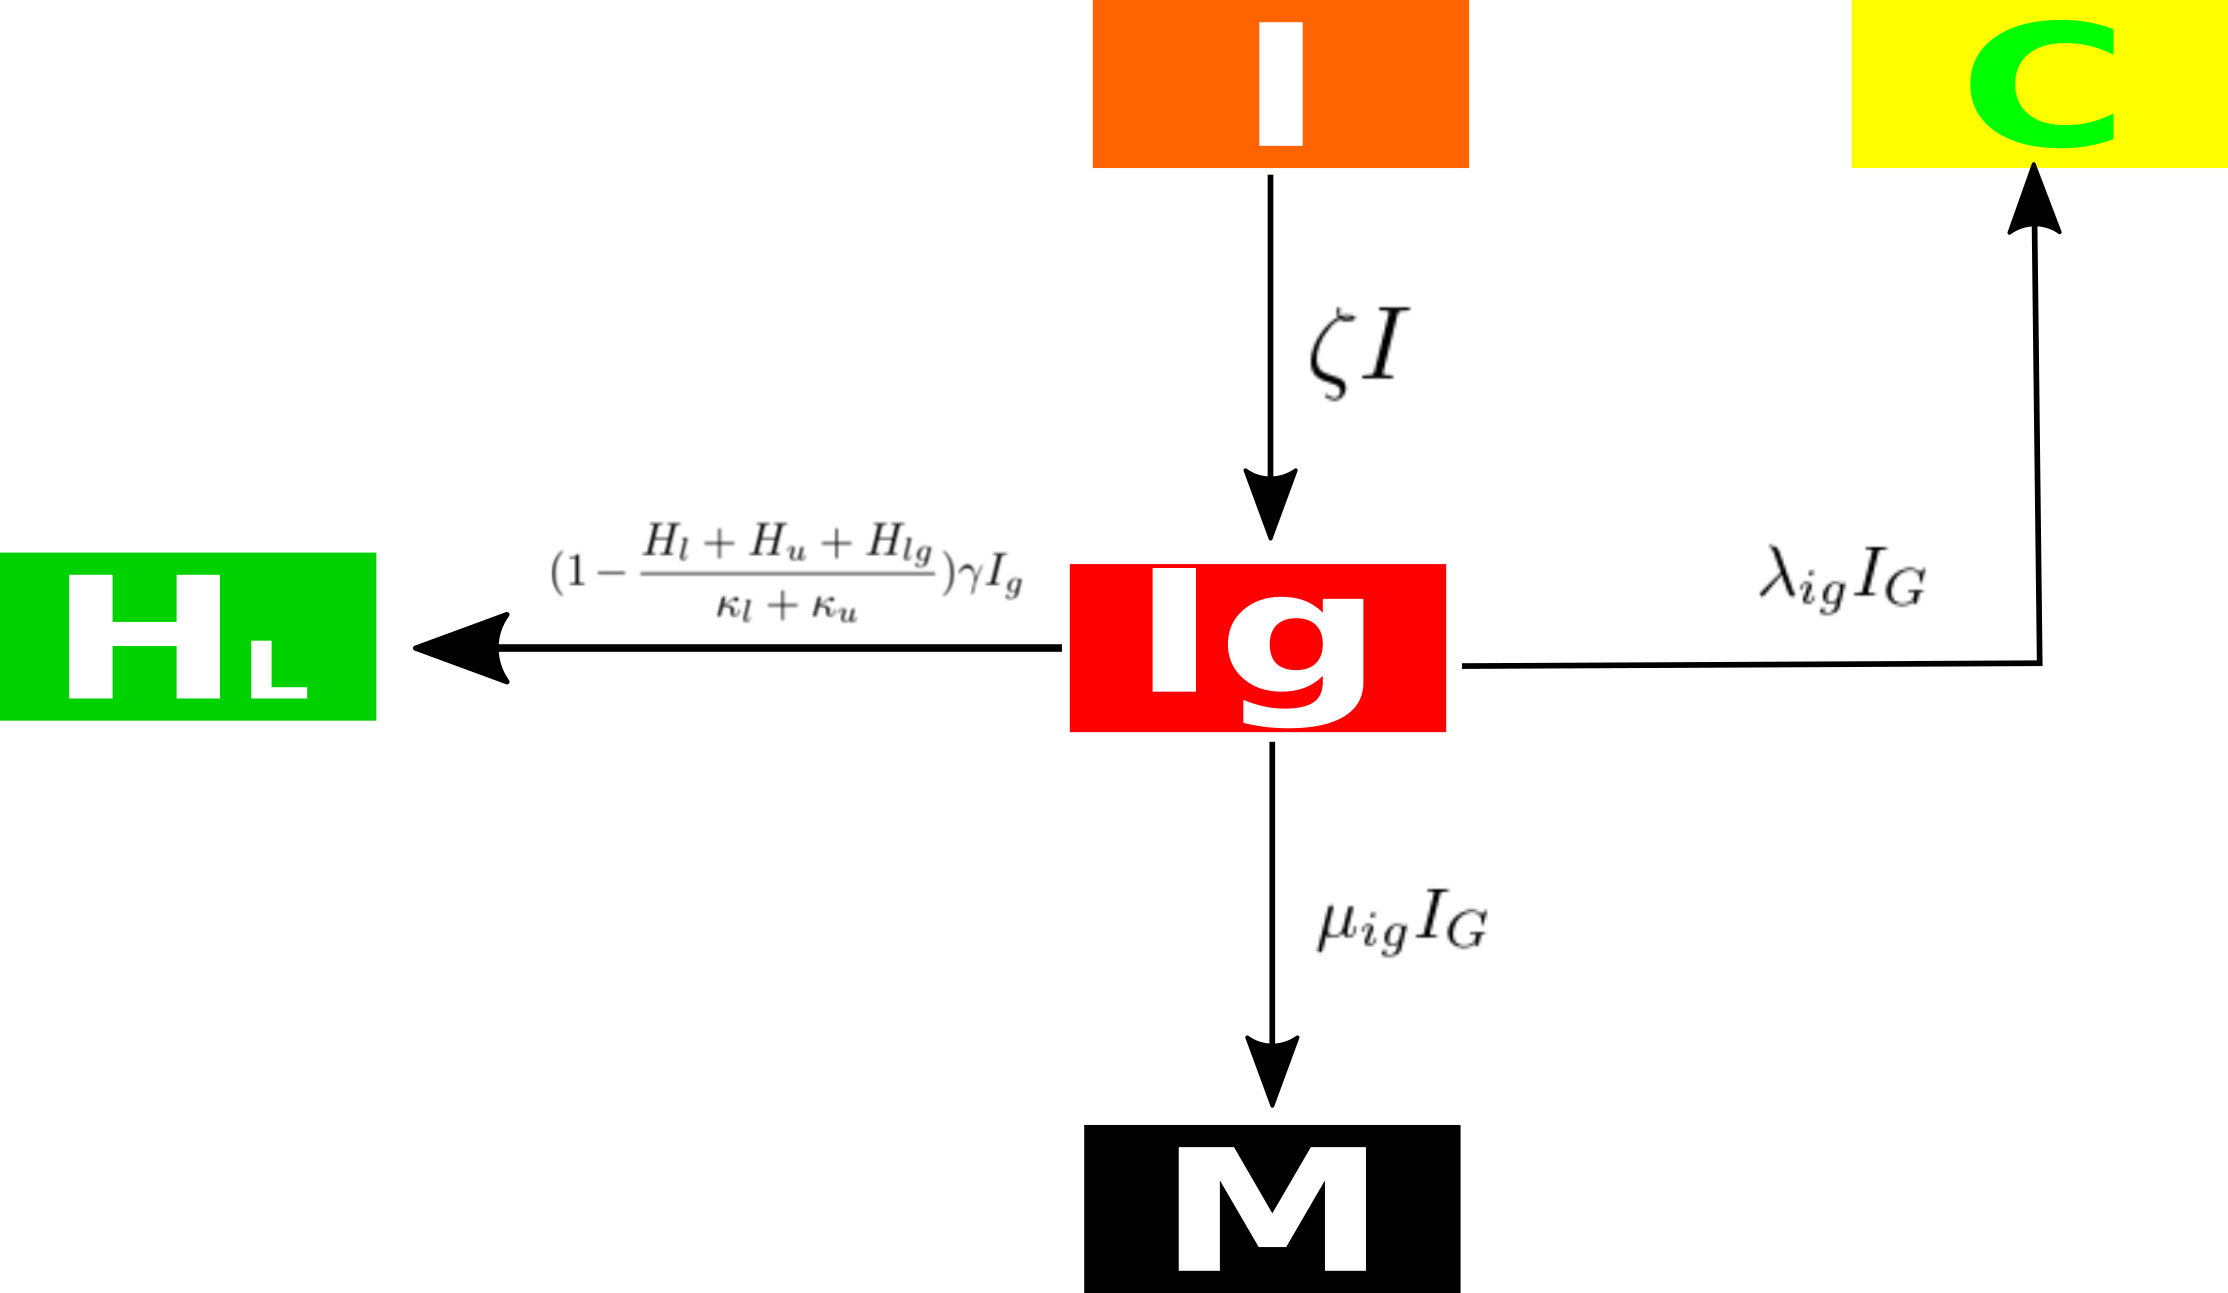
\includegraphics[scale=0.4]{covidIg}
% 	\caption{Diagrama da equação dos Infectados Graves.}
% 	\label{fig:universe}
% \end{figure}
% \subsection{Hospitalizados em Leito Comum ($H_l$)}
% Uma vez hospitalizado, o indivíduo vai para um leito comum e dentro do hospital ele pode seguir alguns caminhos a depender da evolução da doença. Alguns pacientes se curam a uma taxa $\lambda_{hl}$. Outros pacientes irão evoluir para um estado grave, necessitando da internação em UTI. A taxa de agravamento do paciente é $\nu_u$. Além disso, todos os pacientes em estado mais graves não se curam automaticamente. Antes de saírem do hospital esses pacientes retornam para o leito comum. Assim, o número de hospitalizados em leito comum, recebe os indivíduos que estavam hospitalizados em nível mais graves a taxas $\lambda$.
% \begin{equation}
% 	\frac{dH_l}{dt}=(1-\frac{H_l+H_u+H_{lg}}{\kappa_l+\kappa_u})\gamma I_g - \lambda_{hl} H_l - \nu_uH_l + \lambda_{hu}H_u +\lambda_{lg}H_{lg} +\lambda_{lv}H_{lv}
% \end{equation}
% \begin{figure}[!h]
% 	\centering
% 	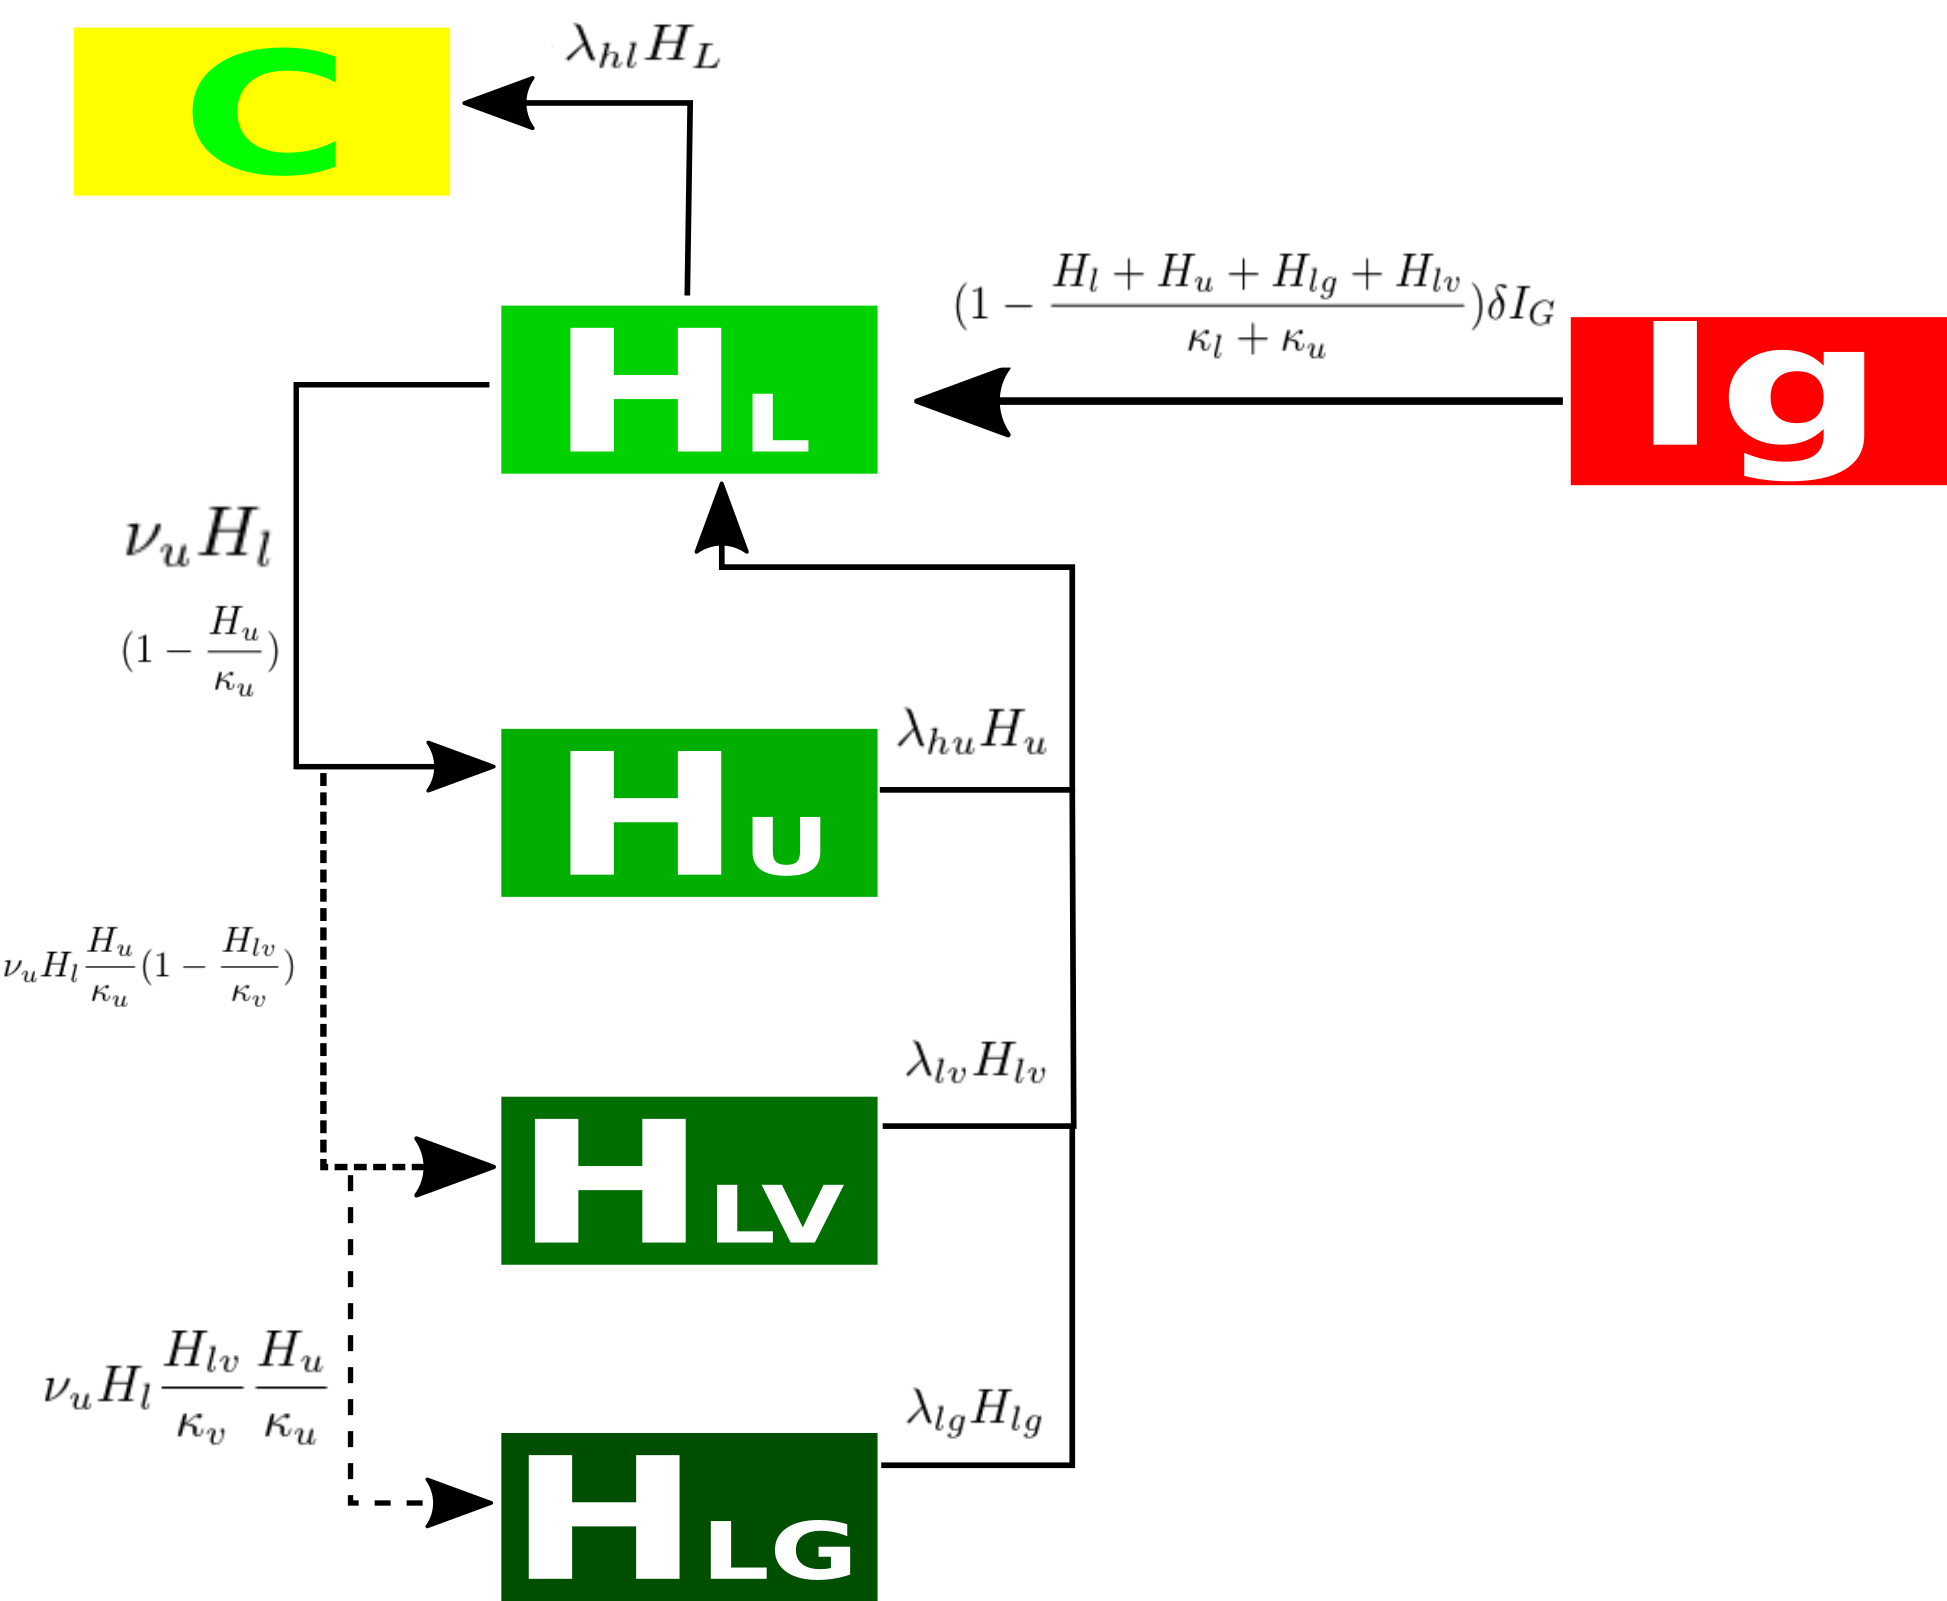
\includegraphics[scale=0.3]{covidHl}
% 	\caption{Diagrama da equação dos Hospitalizados em Leito Comum.}
% 	\label{fig:universe}
% \end{figure}

% \subsection{Hospitalizados em Leito de UTI ($H_u$)}
% Os leitos de UTI são para aqueles que estiveram em leito comum, mas houve o agravamento da situação. A taxa de agravamento do leito comum para o estado grave é $\nu_u$. Contudo, apenas uma fração desses pacientes podem ser recebidos pela UTI. Essa fração é definida pela capacidade de leitos na UTI $\kappa_u$. Não havendo leitos na UTI, estes são direcionados para os níveis mais críticos (Leitos comuns com ventilador mecânico $H_{lv}$ ou apenas leitos comuns com pacientes em estado grave $H_{lg}$). Além disso, o indivíduo pode melhorar, voltando ao leito comum, com taxa $\lambda_{hu}$ ou morrer com taxa $\mu_{hu}$.
% \begin{equation}
% 	\frac{dH_u}{dt}=\nu_u H_l(1 - \frac{H_u}{\kappa_{u}}) -\lambda_{hu} H_u -\mu_{hu} H_u
% \end{equation}
% \begin{figure}[!h]
% 	\centering
% 	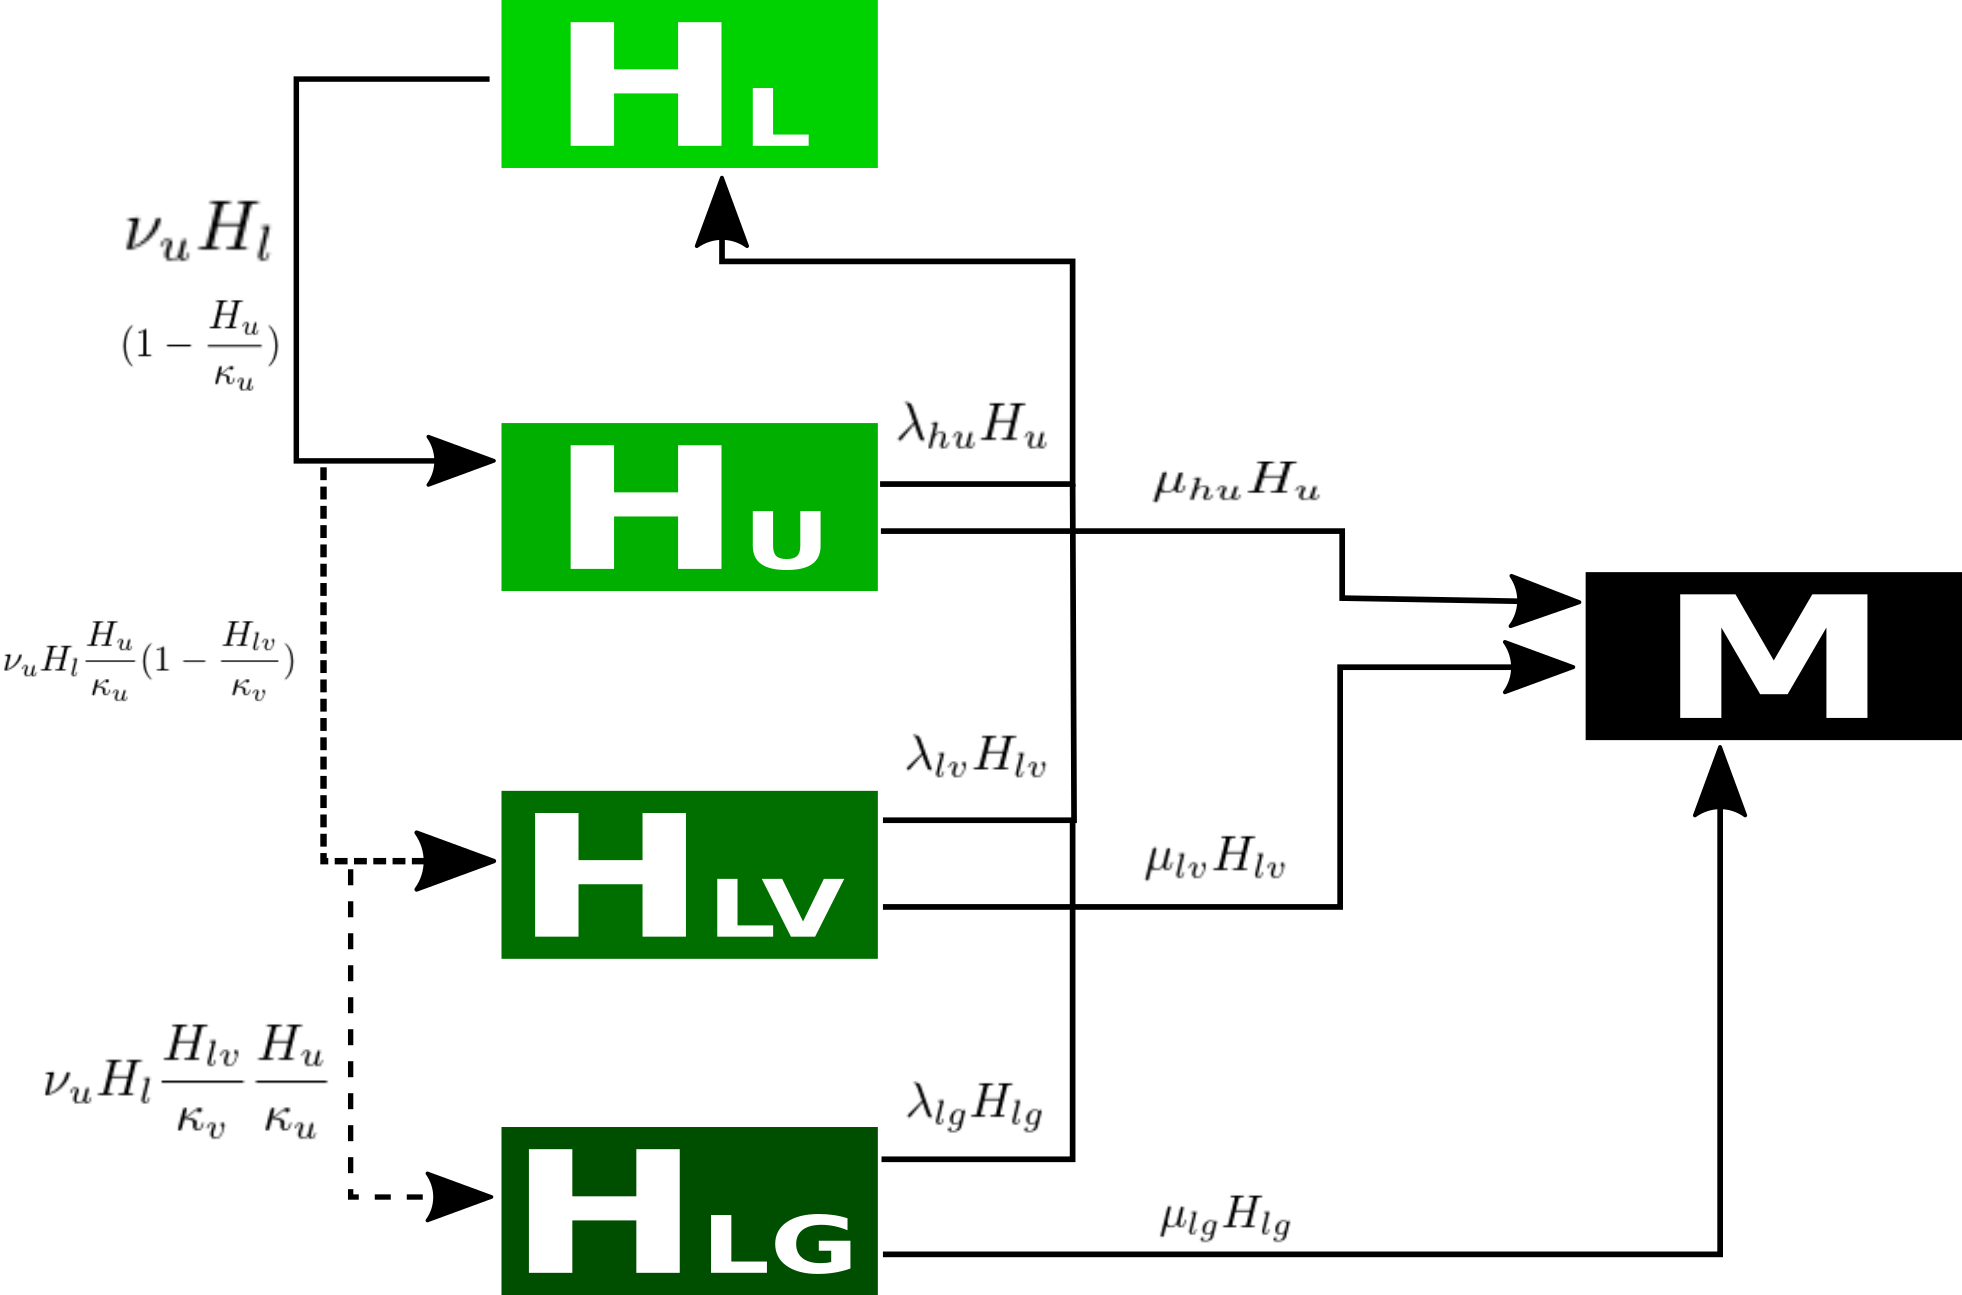
\includegraphics[scale=0.4]{covidHu}
% 	\caption{Diagrama da equação dos Hospitalizados em Estado Grave.}
% 	\label{fig:universe}
% \end{figure}


% \subsection{Hospitalizados em Leito comum com Ventilador Mecânico ($H_{lv}$)}
% Aqueles que tinham que ir para a UTI, mas não conseguiram por falta de leitos, irão para os leitos que possuírem ventiladores mecânicos, até a capacidade de ventiladores mecânicos disponíveis, além dos da UTI ($\kappa_v$). O termo para essa taxa é: $\nu_u H_l \frac{H_u}{\kappa_{u}}(1-\frac{H_{lv}}{\kappa_{v}})$. Além disso, os indivíduos melhoram a uma taxa $\lambda_{lv}$ e morrem a taxas $\mu_{lv}$. Novamente, da prática médica, as taxas de melhoras desses indivíduos são menores dos que estão na UTI.

% \begin{equation}
% 	\frac{dH_{lv}}{dt}=\nu_u H_l\frac{H_u}{\kappa_{u}}(1-\frac{H_{lv}}{\kappa_{v}})  - \lambda_{lv}H_{lv}-\mu_{lv}H_{lv}
% \end{equation}
% \subsection{Hospitalizados em Leito comum em estado grave ($H_{lg}$)}
% Os que não conseguirem ventilador mecânico no leito, ficam em estado grave em um leito comum. Não há necessidade de definir uma capacidade de leitos pois o indivíduo nesse estado já teve seu leito reservado. Além disso, melhoram com uma taxa $\lambda_{lg}$ e morrem a taxa $\mu_{lg}$.

% \begin{equation}
% 	\frac{dH_{lg}}{dt}=\nu_u H_l\frac{H_{lv}}{\kappa_{v}}\frac{H_u}{\kappa_{u}} -\lambda_{lg}H_{lg}-\mu_{lg}H_{lg} 
% \end{equation}

% \subsection{Mortos (M) e Curados (C)}
% Neste modelo, só morrem aqueles que estão em Infectados Graves e os que estão nos hospitais em estados mais graves. Atribuímos que aqueles que estão em leito comum, não morrem. Precisam agravar o caso antes de morrer.

% \begin{equation}
% 	\frac{dM}{dt}=\mu_{ig}I_{g} +\mu_{hl}H_l + \mu_{hu}H_u +\mu_{lv} H_{lv}+\mu_{lg} H_{lg}
% \end{equation}

% Os curados são aqueles que se recuperaram da doença e, enquanto não houver dados contrários, não podem mais ser reinfectados pelo vírus.
% \begin{equation}
% 	\frac{dC}{dt}=\lambda_i I + \lambda_{ig} I_g +\lambda_{hl}H_l 
% \end{equation}

\begin{figure}[!h]
	\centering
	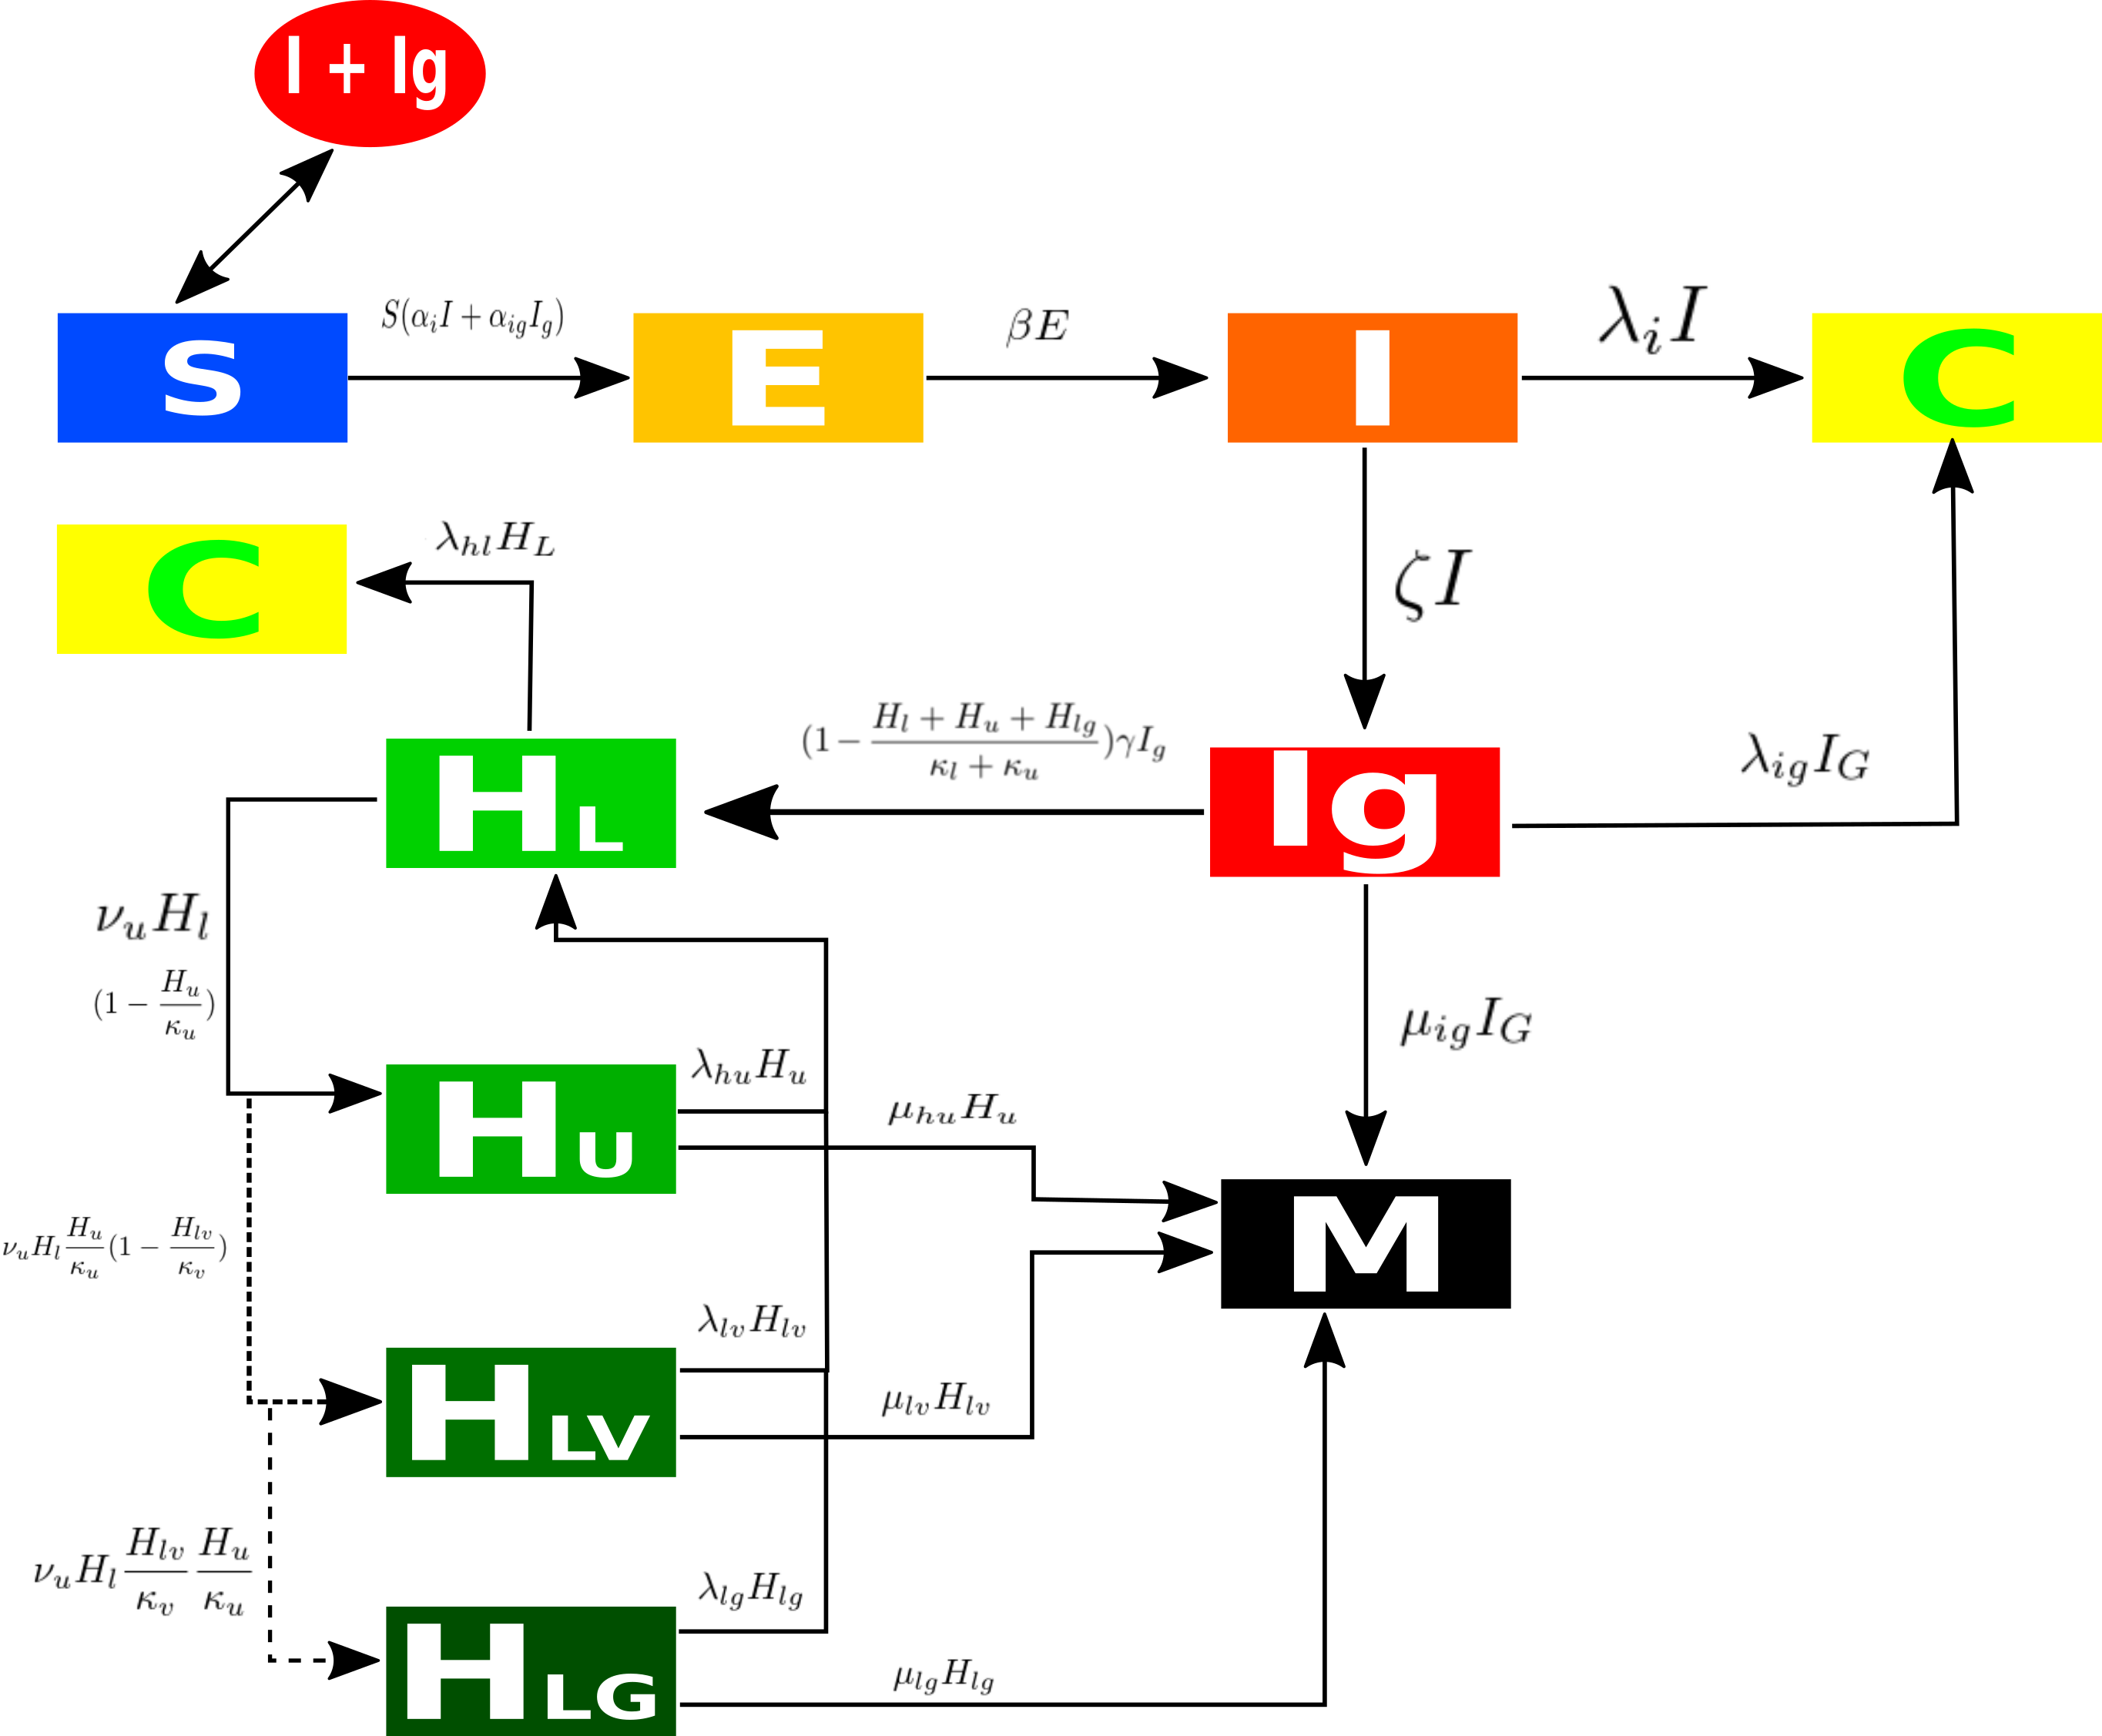
\includegraphics[scale=0.4]{covid}
	\caption{Visão geral dos caminhos para a COVID-19}
	\label{fig:universe}
\end{figure}

\section{Novas Equações}

\begin{equation}
	\frac{dS}{dt}= -S\frac{\delta}{100}(\frac{R_{0i}}{N T_{i}} I +\frac{R_{0ig}}{N T_{ig}}I_g)
\end{equation}
\begin{equation}
	\frac{dE}{dt}= S\frac{\delta}{100}(\frac{R_{0i}}{N T_{i}} I +\frac{R_{0ig}}{N T_{ig}}I_g) - \frac{1}{T_{inc}} E
\end{equation}
\begin{equation}
	\frac{dI}{dt}= \frac{1}{T_{inc}} E -\frac{\lambda_i}{100T_{i}} I - \frac{\zeta}{100T_{i}} I
\end{equation}
\begin{equation}
	\frac{dI_G}{dt}=  \frac{\zeta}{100T_{i}} I -(1-\frac{H_l+H_u+H_{lg}+H_{lv}}{\kappa_l+\kappa_u})\frac{\gamma}{100} I_G - \frac{\lambda_{ig}}{100 T_{ig}} I_G - \frac{\mu_{ig}}{100 T_{ig}} I_G
\end{equation}
\begin{equation}
	% \begin{multlined}
	\frac{dH_l}{dt}=(1-\frac{H_l+H_u+H_{lg}+H_{lv}}{\kappa_l+\kappa_u})\frac{\gamma}{100} I_G - \frac{\lambda_{hl}}{100T_{hl}} H_l - \frac{\nu_u}{100T_{hl}}H_l+ \frac{\lambda_{hu}}{100T_{hu}}H_u +\frac{\lambda_{lg}}{100T_{lg}}H_{lg} +\frac{\lambda_{hv}}{100T_{hv}}H_{lv}
	% \end{multlined}
\end{equation}
\begin{equation}
	\frac{dH_u}{dt}=\frac{\nu_u}{100T_{hl}} H_l(1 - \frac{H_u}{\kappa_{u}}) -\frac{\lambda_{hu}}{100T_{hu}}H_u -\frac{\lambda_{mu}}{100T_{hu}}H_u
\end{equation}

\begin{equation}
	\frac{dH_{lv}}{dt}=\frac{\nu_u}{100T_{hl}} H_l\frac{H_u}{\kappa_{u}}(1-\frac{H_{lv}}{\kappa_{v}})  - \frac{\lambda_{lv}}{100T_{lv}}H_{lv}-\frac{\mu_{lv}}{100T_{lv}}H_{lv}
\end{equation}

\begin{equation}
	\frac{dH_{lg}}{dt}=\frac{\nu_u}{100T_{hl}} H_l\frac{H_{lv}}{\kappa_{v}}\frac{H_u}{\kappa_{u}} -\frac{\lambda_{lg}}{100T_{lg}}H_{lg}-\frac{\mu_{lg}}{100T_{lg}}H_{lg}
\end{equation}
\begin{equation}
	\frac{dM}{dt}=\frac{\mu_{ig}}{100 T_{ig}}I_{g} +\frac{\mu_{hl}}{100 T_{hl}}H_l + \frac{\mu_{hu}}{100 T_{hu}}H_u +\frac{\mu_{lv}}{100 T_{lv}} H_{lv}+\frac{\mu_{lg}}{100 T_{lg}} H_{lg}
\end{equation}
\begin{equation}
	\frac{dC}{dt}=\frac{\lambda_i}{100 T_{i}} I + \frac{\lambda_{ig}}{100 T_{ig}} I_g +\frac{\lambda_{hl}}{100 T_{hl}}H_l 
\end{equation}

Descrição das variáveis, sendo que a notação é [min, max, passo]:
\begin{enumerate}
	\item N - Tamanho da população - Livre
	\item $\delta = [0, 100, 1]$
	\item $R_{0i} = [0, 15, 0.01]$
	\item $R_{0ig} = [0, 15, 0.01]$
	\item $T_{X} = [0, 50, 1]$
	\item $\lambda_X = [0,100, 1]$
	\item $\zeta = [0, 100, 1]$
	\item $kappa_l$ é livre (pode deixar numa caixa para digitar)
	\item  $kappa_u$ é livre (pode deixar numa caixa para digitar)
	\item $\gamma = [0,100, 1]$
	\item $\mu_{X} = [0,100, 1]$
	\item $\nu_u = [0,100,1]$
	      	      	      	      	      	      	      	      	      	      	      	      	      	      	      	      	      	      	      	      	      	      	      	      	      	      	      	      	      	      	      	      	      	      	      	      	      	      	      	      	      	
\end{enumerate}







\subsection{As variáveis do modelo}

\begin{table}[h]
	\begin{tabular}{|c|p{7cm}|p{2cm}|l|l}
		\cline{1-4}
		Símbolo       & Definição                                                                            & Valor Padrão             & Referência &   \\ \cline{1-4}
		$\delta$       & Percentual da população que não está seguindo a quarentena                         &                           &             &   \\ \cline{1-4}
		$\alpha_i$     & Taxa de transmissão entre os infectados e saudáveis                                  & 3/14 Cada I contamina 3 S &             &   \\ \cline{1-4}
		$\alpha_{ig}$  & Taxa de transmissão entre os infectados graves e saudáveis                           &                           &             &   \\ \cline{1-4}
		$\beta$        & Taxa de conversão dos Expostos em Infectados (ativos)                                 & 1/14                      &             &   \\ \cline{1-4}
														
		$\lambda_I$    & Taxa de Cura do indivíduo Infectado                                                   &                           &             &   \\ \cline{1-4}
		$\zeta$        & Taxa de evolução dos infectados para o estado grave                                  &                           &             &   \\ \cline{1-4}
		$\gamma$       & Percentual dos que estão em estado grave e procuram o hospital                        &                           &             &   \\ \cline{1-4}
		$\lambda_{ig}$ & Taxa de Cura do indivíduo Infectado grave                                             &                           &             &   \\ \cline{1-4}
		$\mu_{ig}$     & Taxa de morte do indivíduo Infectado grave                                            &                           &             &   \\ \cline{1-4}
		$\lambda_{hl}$ & Taxa de Cura do indivíduo hospitalizado em leito comum                                &                           &             &   \\ \cline{1-4}
		$\lambda_{hu}$ & Taxa de melhora do indivíduo hospitalizado  na UTI                                    &                           &             &   \\ \cline{1-4}
		$\mu_{hu}$     & Taxa de morte do indivíduo hospitalizado  na UTI                                      &                           &             &   \\ \cline{1-4}
		$\lambda_{lg}$ & Taxa de melhora do indivíduo hospitalizado  em leito comum e no estado grave          &                           &             &   \\ \cline{1-4}
		$\mu_{lg}$     & Taxa de morte do indivíduo hospitalizado  em leito comum e no estado grave            &                           &             &   \\ \cline{1-4}
		$\lambda_{lv}$ & Taxa de melhora do indivíduo hospitalizado  em leito comum e com ventilador mecânico &                           &             &   \\ \cline{1-4}
		$\mu_{lv}$     & Taxa de morte do indivíduo hospitalizado  em leito comum e com ventilador mecânico   &                           &             &   \\ \cline{1-4}
		$\nu{u}$       & Taxa de agravamento do indivíduo hospitalizado em leito comum                         &                           &             &   \\ \cline{1-4}
		$\kappa_u$     & número de leitos de UTI                                                               &                           &             &   \\ \cline{1-4}              
		$\kappa_l$     & número de leitos comuns                                                               &                           &             &   \\ \cline{1-4}              
		$\kappa_v$     & número de ventiladores disponíveis  além dos utilizados nas UTIs                    &                           &             &   \\ \cline{1-4}        
	\end{tabular}
	\caption{ Variáveis do modelo}
\end{table}

	
% https://ciis.fmrp.usp.br/covid19/epcalc/public/index.html
	
% \section{Conclusion}
	
% \bibliographystyle{plain}
% \bibliography{references}
\end{document}
